\documentclass[12pt]{article}
\usepackage[spanish]{babel}
\usepackage{url}
\usepackage[utf8x]{inputenc}
\usepackage{blindtext}
\usepackage{amsmath}
\usepackage{graphicx}
\usepackage{float}
\graphicspath{{images/}}
\usepackage{parskip}
\usepackage{fancyhdr}
\usepackage{vmargin}
\setmarginsrb{3 cm}{2.5 cm}{3 cm}{2.5 cm}{1 cm}{1.5 cm}{1 cm}{1.5 cm}

\title{Decide Ortosia - Autenticación}								%Title
								% Author
\date{12 Sept 2015}											% Date

\makeatletter
\let\thetitle\@title
\let\theauthor\@author
\let\thedate\@date
\makeatother

\pagestyle{fancy}
\fancyhf{}
\rhead{\theauthor}
\lhead{\thetitle}
\cfoot{\thepage}

\begin{document}

%%%%%%%%%%%%%%%%%%%%%%%%%%%%%%%%%%%%%%%%%%%%%%%%%%%%%%%%%%%%%%%%%%%%%%%%%%%%%%%%%%%%%%%%%

\begin{titlepage}
	\centering
    \vspace*{0.5 cm}
    
\includegraphics[scale = 0.2]{logo.png}\\[1.0 cm]	% University Logo
    \textsc{\LARGE Escuela Técnica Superior de Ingeniería  \newline\newline Informática}\\[2.0 cm]	% University Name
	\textsc{\Large Opera Id:125}\\[0.5 cm]				% Course Code
	\rule{\linewidth}{0.2 mm} \\[0.4 cm]
	{ \huge \bfseries \thetitle}\\
	\rule{\linewidth}{0.2 mm} \\[1.5 cm]
	
	\begin{minipage}{0.4\textwidth}
		\begin{flushleft} \large
			\emph{Autores:}\\
			Álvaro González \\		
			Luca Bonacini\\
            Antonio Millan \\
            Rodrigo Rojas \\
            Antonio Romero \\
			\end{flushleft}
			\end{minipage}~
			\begin{minipage}{0.4\textwidth}
            
			\begin{flushright} \large
			\emph{Tutores:} \\
			David Benavides Cuevas\\
            \emph{Opera Id: }
            125\\
			\emph{Grupo: }            
            G1\\
            
            
		\end{flushright}
        
	\end{minipage}\\[2 cm]
	
	
    
    
    
    
	
\end{titlepage}

%%%%%%%%%%%%%%%%%%%%%%%%%%%%%%%%%%%%%%%%%%%%%%%%%%%%%%%%%%%%%%%%%%%%%%%%%%%%%%%%%%%%%%%%%

\tableofcontents
\listoffigures
\listoftables
\pagebreak

%%%%%%%%%%%%%%%%%%%%%%%%%%%%%%%%%%%%%%%%%%%%%%%%%%%%%%%%%%%%%%%%%%%%%%%%%%%%%%%%%%%%%%%%%

\section{Resumen}
Decide es una herramienta Open Source que se desarrolla con el fin de facilitar el voto online de manera segura, anonima y eficaz. Decide es un software heredado realizado por el equpo de Wadobo \url{https://github.com/wadobo/decide}.
En un primer momento se realizó un fork de este sistema para que podamos trabajar de forma aislada sin tener que modificar el sistema original.
El sistema se divide en varios subsistemas para facilitar el escalado y el mantenimiento del software. Dichos subsistemas se comunican entre ellos a través de llamadas REST.  


Nuestro grupo se encarga del subsistema de autenticación. Es el primer paso  para que un usuario pueda votar, garantizar que la persona que va a realizar el voto es quien dice ser. Como se ha comentado previamente el codigo fuente es heredado por lo que teniamos que seguir el lenguaje, estrategia y estructura que se había definido en un principio. El equipo decidió no desarrollar el subsistema con otra tecnologia ya que podría afectar al buen funcionamiento del sistema y podríamos encontrarnos con conflictos con los resto de subsistemas.  


Despues el equipo llego a un acuerdo sobre las tareas que se iban a desarrollar a lo largo del proyecto entre los que se encuentran distintos métodos de autenticación, documentación de la API, interfaz de usuario, etc. Cada miembro del equipo tenia asignadas unas tareas (\emph{issues}) y para gestionar el codigo se ha usado un repositorio GIT con el fin de que tuvieramos siempre la última versión del sistema (tanto por nuestra parte como con el resto de los equipos) y poder resolver conflictos de una forma mas eficiente.



\newpage	
\section{Introducción y contexto}

Es un proyecto para que el equipo de trabajo ponga en práctica y observe cómo se ponen en funcionamiento un proyecto real, en este caso se trabaja con Decide que es una plataforma didáctica de votación electrónica.

En el proyecto definimos diferentes subsistemas que serán más o menos independientes entre sí y que se interconectan implementando una API concreta.
Cada subsistema se encarga de una tarea concreta en el sistema de voto. Los subsistemas a realizar son los siguientes \cite{decide-subsistemas}

 \begin{enumerate}
    \item Autenticación
    \item Censo
    \item Votaciones
    \item Cabina de votación
    \item Almacenamiento de votos (cifrados)
    \item Recuento/ MixNet
    \item Post-procesado
    \item Visualización de resultados
 \end{enumerate}

Nuestro equipo se encargará del subsistema de autenticación que consistirá en autenticar al votante (con esto nos referimos a que se verifique que realmente la persona que vota dice ser quién es sin que se de el caso de suplantación de identidad), y que el votante solo pueda votar una vez en esa votación.


\section{Descripción del sistema}

\section{Planificación del proyecto}
Para la planificación del proyecto el equipo tuvo una reunión al principio del milestone para discutir y llegar a un acuerdo en las tareas que se iba a realizar durante el desarrollo del mismo. Las tareas estan definidas en el apartado de issues del repositorio \url{https://github.com/pablotabares/decide/issues} cada tarea tiene asignada una/s persona/s que seran los repsonsables de que dicha tarea se lleve a cabo en tiempo y en forma. 

Para gestionar el tiempo que ha dedicado cada miembro del equipo hemos utilizado la herramienta Toggle \cite{toggl} y se han incluido los reportes en el diario del equipo. 

Debido a que uno de los miembros se encuentra fuera de Sevilla y debe trabajar de forma remota el equipo llego a un acuerdo de reunirse los miercoles para conocer los avances y problemas que ha tenido el proyecto. Además se usaría Telegram \cite{telegram} como herramienta de comunicación de forma diaria.

\section{Entorno de desarrollo}
Nuestra primera aproximación fue usar como entorno de desarrollo Docker ya que este sería tambien el entorno de producción. Sin embargo, encontramos una serie de problemas para cumplir con este objetivo. El primero fue que los cambios que se hicieran en local tenían que verse reflejados en la imagen de Docker y por tanto actualizarse sin problemas. Para ello había que cambiar y configurar el Dockerfile y usar Volumes \cite{update-code-docker}. Logramos que los cambios se producesen pero no nos era posible debugear el codigo. 

Finalmente optamos por la otra alternativa que aparece en el repositorio principal. Que consta de las siguientes tecnologias:

\begin{itemize}
\item Python 3.6.5
\item Django 3.7.7
\item PostgresSQL 10.6
\item Pycharm Studio Professional 2018
\end{itemize}

Decidimos usar Pycharm Studio Professional ya que la Universidad de Sevilla cuenta con una licencia para estudiantes \cite{github-student}, por lo que tiene mas soporte y más caracteristicas que Pycharm Studio Community. Además se puede configurar un entorno de Django desde el mismo IDE para que el desarrollo sea más efectivo.


\section{Gestión del cambio, incidencias y depuración}

Las incidencias y cambios en el sistema se deben publicar en el apartado de  \emph{issues} en el repositorio del proyecto. Ya que estamos trabajando con otros subsistemas y otros equipos se propone que el titulo de la incidencia debería comenzar con Auth seguido de la incidencia o cambio propuesto. Por ejemplo: Auth - Email authentication \cite{auth-issue}

Además se debe indicar la persona responsable, una etiqueta, proyecto asociado y si es posible indicar el milestone como se muestra en la siguiente imagen:

\begin{figure}[h]
\centering
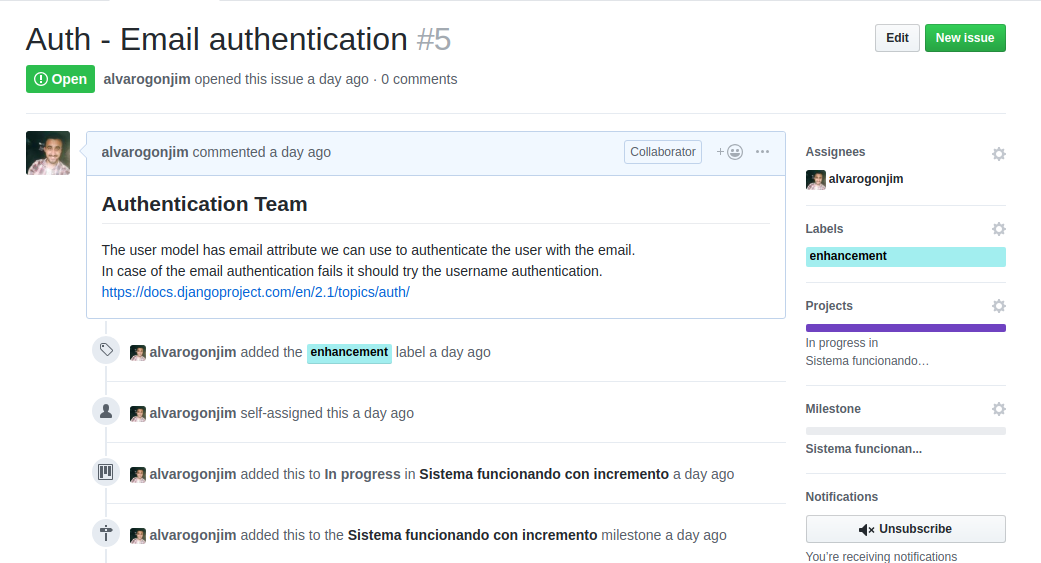
\includegraphics[width=1\textwidth]{issue-example.png}
\caption{Ejemplo de incidencia}
\end{figure}

\newpage
\subsection{Gestión del código fuente}
La gestión del código fuente de nuestro proyecto se hará a través de Git ya sea por comandos (en la terminal) o a través de una interfaz de usuario. 
Los commits deben seguir la siguiente estructura \cite{commit-structure}:

Titulo: Extracto de los cambios en 50 caracteres o menos.

Texto explicativo más detallado, solo si es necesario. La línea en blanco que separa el titulo del resto del texto es crucial.
En el pie, se pueden poner referencias (ids) de las incidencias.

\begin{figure}[h]
\centering
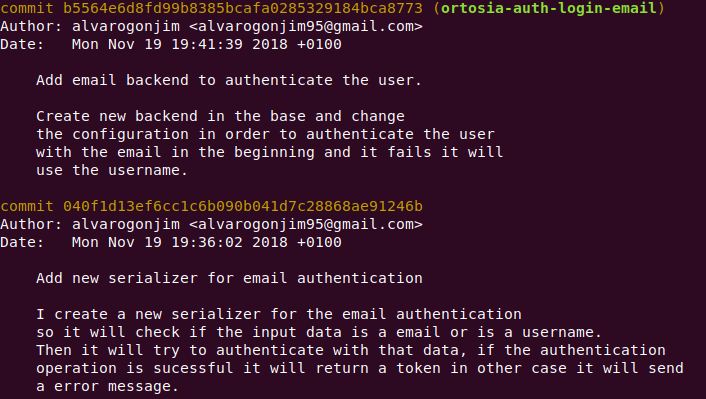
\includegraphics[width=0.8\textwidth]{commits.png}
\caption{Ejemplo de estructuras de commits}
\end{figure}

Para la gestión de ramas se empleará una rama por incidencia (aunque la incidencia sea muy leve o facil de realizar). El estructura de la rama debe ser ortosia-auth-\emph{titulo de la incidencia} como por ejemplo se puede ver en la imagen previa \emph{ortosia-auth-login-email}

Una vez que se haya finalizado el desarrollo de la incidencia se debe realizar un \emph{Pull Request (PR)} a la rama ortosia-auth. Este PR debe ser revisado por una/s persona/s que no sean los responsables y/o desarrolladores de la incidencia. En caso de que apruebe el PR se mergeara, en caso contrario, el responsable deberá realizar los cambios propuestos. 

\begin{figure}[hbt!]
\centering
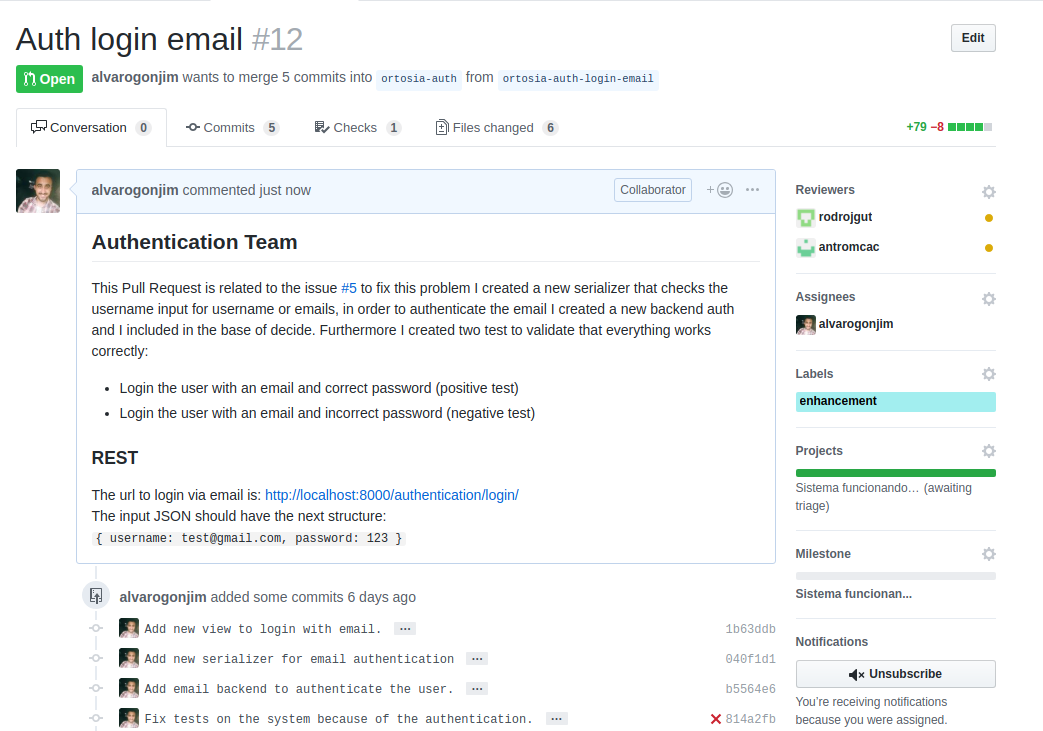
\includegraphics[width=0.8\textwidth]{pr.png}
\caption{Ejemplo de Pull Request a ortosia-auth}
\end{figure}

\begin{figure}[hbt!]
\centering
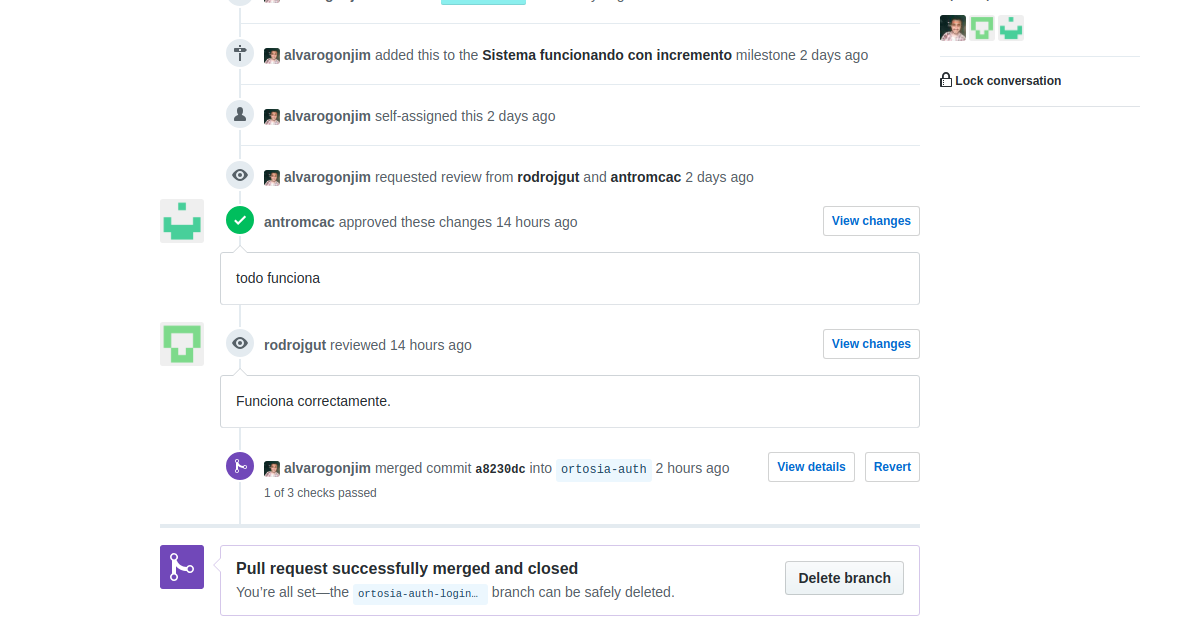
\includegraphics[width=0.8\textwidth]{approved.png}
\caption{Ejemplo de Pull Request revisado y aprobado}
\end{figure}


Cuando la rama base de nuestro equipo (ortosia-auth) sea estable y no tenga  fallos ni conflictos se realizará un PR a la rama master y posteriormente el proceso de despligue. 



\subsection{Gestión de la construcción e integración continua}
El proyecto que estamos realizando va ser desplegado en un servidor remoto. Para la integración continua usaremos Travis CI.
Travis CI es un servicio de integración continua distribuido y alojado que se utiliza para crear y probar proyectos de software alojados en GitHub. Travis CI recoge el código de nuestra aplicación, lo compila y realiza una serie de test con el fin de probar que funciona correctamente.
Una vez registrados en Travis CI, procedemos a sincronizado el repositorio de GitHub que vamos a utilizar, creamos un archivo llamado .travis.yml en la raíz de nuestro proyecto. Éste archivo contiene una serie de comandos para hacer que los test funcionen y así poder comprobar el buen funcionamiento de nuestro proyecto.
Travis CI detecta los cambios automaticamente, pasa los tests y construye el proyecto con los cambios realizados en el repositorio.

\begin{figure}[hbt!]
\centering
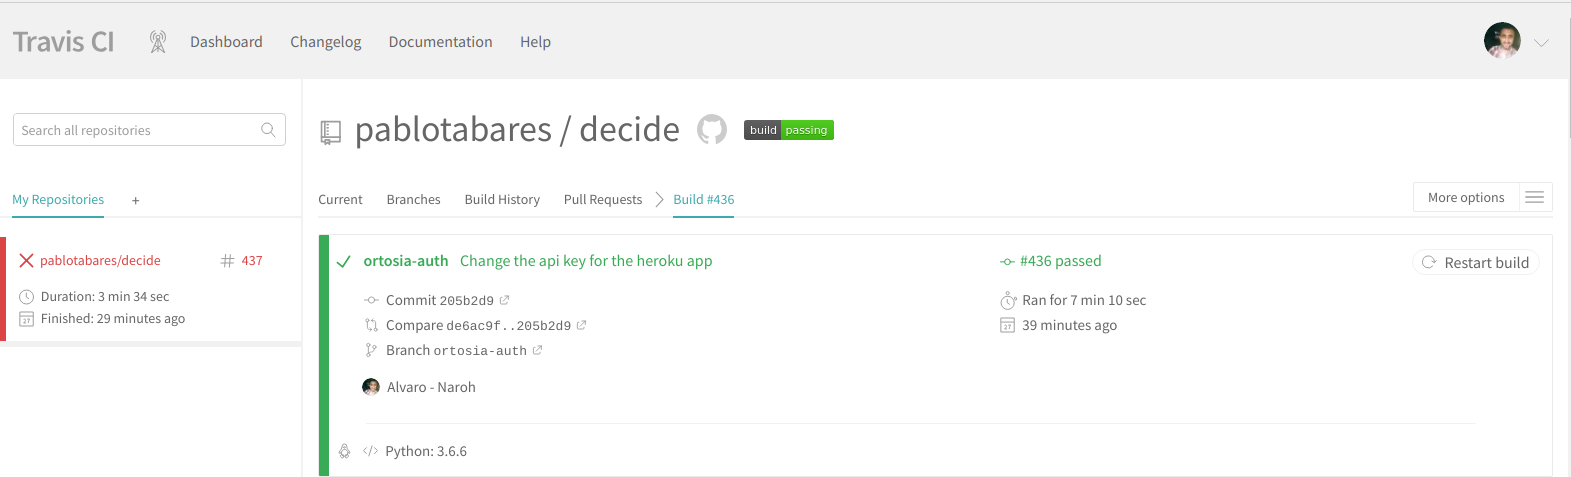
\includegraphics[width=1\textwidth]{travis.png}
\caption{Ejemplo de construcción con Travis CI}
\end{figure}


\subsection{Gestión de liberaciones, despliegue y entregas}

Para desplegar el proyecto se va a usar Heroku. Heroku es una plataforma como servicio que permite desplegar y operar aplicaciones en la nube sin ningun problema de forma gratuita.
Además se puede configurar con Travis CI para que el proceso de despliegue se realice de forma automatica cuando exista algun cambio en la rama correspondiente. De esta forma nosotros vamos a desplegar nuestro subsistema de forma aislada desde nuestra rama base ortosia-auth
Mientras que para el sistema completo con todos los subsistemas se va a usar la rama master.

Para crear una aplicación de Heroku tenemos que crearnos una cuenta en su pagina principal \url{https://www.heroku.com}. Luego hacemos click en "Crear una nueva App" definimos un nombre para la nueva app y en la siguiente ventana nos explicará como desplegar el proyecto en esta nueva app a través de Heroku CLI. Sin embargo nosotros usamos Travis CLI (para un despliegue automatico), debemos crear un fichero Procfile que determina que acción/es debe realizar Heroku cuando se suba el proyecto y tambien debemos modificar el travis.yml con una sección de despliegue como en el siguiente ejemplo:

\begin{figure}[hbt!]
\centering
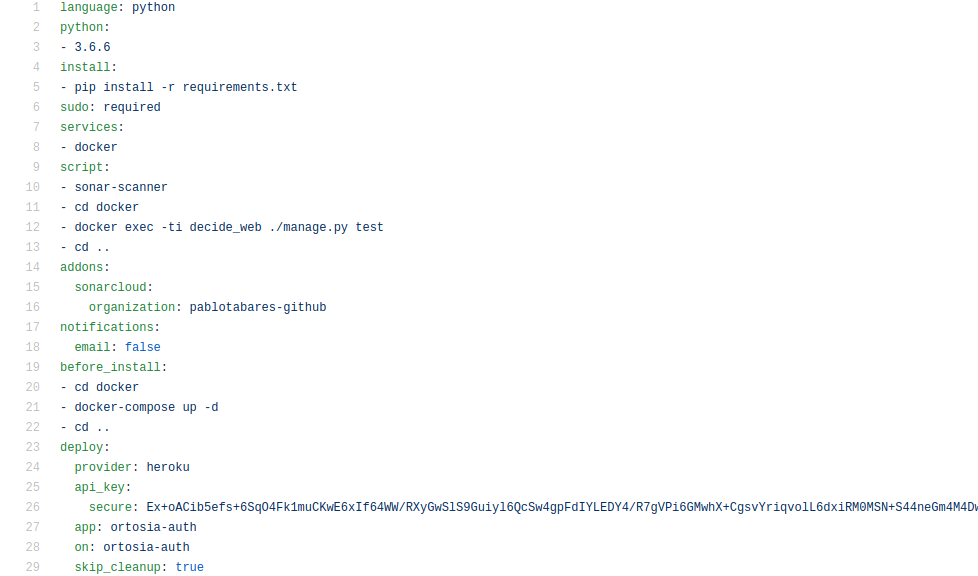
\includegraphics[width=1\textwidth]{travisyml.png}
\caption{Resultado de travis.yml tras añadir la sección de despliegue}
\end{figure}

Se puede apreciar en la sección deploy que el cliente que vamos a usar es Heroku. El nombre de la aplicación debe coincidir con el que hemos creado previamente (ortosia-auth) y podemos indicar sobre que rama queremos que tome los cambios gracias al atributo 'on'. 
Podemos ver en la imagen que hay una clave de seguridad, esta clave se puede obtener edsde nuestro perfil de Heroku en la sección API Key, pero debemos encriptar dicha API Key con el comando

\verb|travis encrypt $(heroku auth:token)--add deploy.api_key|
\cite{heroku-deployement}


\begin{table}[H]
\begin{tabular}{lllll}
\cline{1-4}
\multicolumn{1}{|l|}{Sistema} & \multicolumn{1}{l|}{URL} & \multicolumn{1}{l|}{Usuario} & \multicolumn{1}{l|}{Contraseña} &  \\ \cline{1-4}
\multicolumn{1}{|l|}{Autenticación} & \multicolumn{1}{l|}{https://ortosia-auth.herokuapp.com} & \multicolumn{1}{l|}{administrator} & \multicolumn{1}{l|}{Admin2018.} &  \\ \cline{1-4}
\multicolumn{1}{|l|}{} & \multicolumn{1}{l|}{} & \multicolumn{1}{l|}{} & \multicolumn{1}{l|}{} &  \\ \cline{1-4}
                       &                       &                       &                       & 
\end{tabular}
\caption{Sistemas desplegados en Heroku}
\end{table}

\section{Mapa de herramientas}

Para el desarrollo hemos realizado el proyecto con django y postgressql. Dicho proyecto se sube a un repositorio (decide) en comun con el resto de equipos. Los subsistemas estaban aislados ya que cada uno tiene su rama propia. Cada vez que hay algun cambio en Github se pasa a la integración continua gracias a Travis CI, este lanza los test de calidad con SonarQube y se construye el proyecto con Docker. En caso de error se notifica al equipo de desarrollo para que solucionen el problema. Si no hay errores y la construcción del proyecto se ha realizado de forma satisfactoria Travis despliega el proyecto en Heroku donde se puede acceder desde cualquier dispositivo.

\begin{figure}[hbt!]
\centering
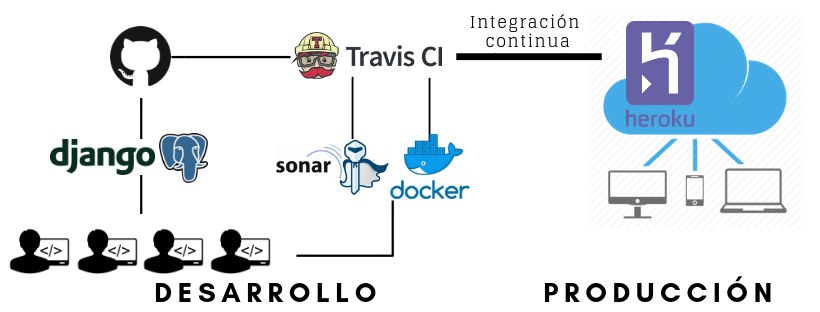
\includegraphics[width=1\textwidth]{Desarrollo.png}
\caption{Mapa de herramientas}
\end{figure}


\section{Ejercicio de propuesta de cambio}
En esta sección vamos a explicar un cambio desde 0 incluyendo todos los pasos que deberiamos de realizar para llevarlo desde el desarrollo hasta la fase de producción.

El primer paso sería clonar el proyecto de Github:

\emph{\$ git clone 
https://github.com/pablotabares/decide.git}

Una vez hecho esto, será necesario instalar las dependencias del proyecto, las cuales están en el fichero requirements.txt:

\emph{\$ pip install -r requirements.txt}

Tras esto tendremos que crearnos nuestra base de datos con postgres:

\emph{\$ sudo su - postgres}

\emph{psql -c "create user decide with password 'decide'"}

\emph{psql -c "create database decide owner decide"
}

Entramos en la carpeta del proyecto y realizamos la primera migración para preparar la base de datos que utilizaremos:

\emph{\$ cd decide
\$ python manage.py migrate
}

El cambio que proponemos es el de aumentar el numero de atributos que tiene el objeto user. El primer paso que debemos hacer es crear una issue tal como se vió en el apartado de la gestion del código fuente. Esta issue fue reportada en el siguiente url:

\url{https://github.com/pablotabares/decide/issues/52}

Ahora lo que vamos a hacer es crear una rama siguiendo el estilo anteriormente descrito que sera donde vamos a trabajar en esta issue, para ello usamos el comando:

\emph{\$ git checkout -b ortosia-auth-model-decideuser}


Ahora podemos trabajar en la issue, sin problemas. 
Cuando hayamos terminado con los cambios en el desarrollo debemos subir el código y posteriormente hacer un PR a nuestra rama base, para ello debemos de usar el comando:

\emph{\$ git add .}

\emph{\$ git commit .}

\emph{\$ git push origin ortosia-auth-model-decideuser}

Cuando hayamos terminado podemos crear un pull request para ello debemos ir a Github a nuestra rama (ortosia-auth-model-decideuser) y hacer click en new pull request, nosotros ya hemos realizado el PR en la siguiente url; \url{https://github.com/pablotabares/decide/pull/174}

Nuestro compañero validará el pull request o nos pedirá distintos cambios y en caso de que el pull request sea aceptado podremos mergearlo a nuestra rama base (ortosia-auth). 

Ahora si entramos en la web de TravisCI y entramos en la rama de ortosia-auth podemos ver en el fichero de log como se pasán los test unitarios, de calidad de código (SonarQube) y si no hay problemas se desplegará una nueva versión en Heroku. Esto se realiza de forma automatica, no tenemos que preocuparnos de nada. En nuestro caso podemos visualizar dichos resultados en el siguiente enlace:

\url{https://travis-ci.org/pablotabares/decide/builds/478420406}

Gracias al fichero Postman que hemos realizado podemos hacer una consulta y comprobar que el cambio que hemos realizado funciona sin problemas.

\begin{figure}[h]
\centering
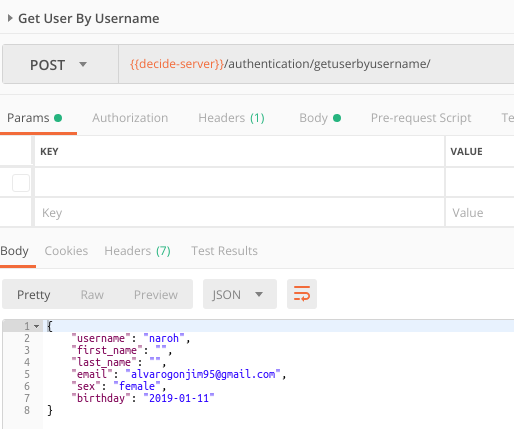
\includegraphics[width=1\textwidth]{call.png}
\caption{Ejemplo de incidencia}
\end{figure}

Como se puede ver en la figura, aparecen todos los datos del usuario ademas de los atributos de sexo y fecha de nacimiento.

\section{Conclusiones y trabajo futuro}

Como conclusiones finales, consideramos que el proycto se ha realizado de forma exitosa. Se han seguido los procedimientos definidos en este documento para llevar el proyecto a cabo.

Añadir que el equipo ha aprendido nuevas tecnologias y metodologías para que el desarrollo de un producto sea lo mas eficiente posible, gracias a la integración continua, el uso de tests unitarios, test de calidad hasta llevarlo a una fase de producción.

Por último, como trabajo futuro se pueden añadir nuevas funcionalidades al modulo de autenticación como por ejemplo:

\begin{enumerate}
\item Autenticación con redes sociales
\item Autenticación a traves de un servidor LDAP
\item Autenticación via SMS o aplicaciones de mensajería.
\item Incrementar numero de tests para que la cobertura de código sea mayor.
\end{enumerate}

\newpage	


\begin{thebibliography}{9}
\bibitem{decide-subsistemas} 
Dani GM
\textit
{https://github.com/EGCETSII/decide/blob/master/doc/subsistemas.md}

\bibitem{update-code-docker}
Bialba, 21 Septiembre 2016. 
\textit{https://stackoverflow.com/questions/39615405/updating-code-in-a-docker-container/}

\bibitem{toggl} 
\textit{https://toggl.com/}

\bibitem{telegram} 
\textit{https://web.telegram.org/}

\bibitem{github-student} 
\textit{https://education.github.com/pack}

\bibitem{auth-issue} 
\textit{https://github.com/pablotabares/decide/issues/5}

\bibitem{heroku} 
\textit{https://www.heroku.com/}

\bibitem{commit-structure}
Miguel Angel Bueno Ferrer, 23 Abril 2017. 
\textit{https://blog.kirei.io/}

\bibitem{heroku-deployement}
\textit{https://docs.travis-ci.com/user/deployment/heroku/}




\end{thebibliography}


\end{document}